\documentclass{standalone}
%outline around text
\usepackage[outline]{contour}
\contourlength{1.3pt}

%tikz
\usepackage{tikz}
\usetikzlibrary{knots, cd, calc}

\begin{document}

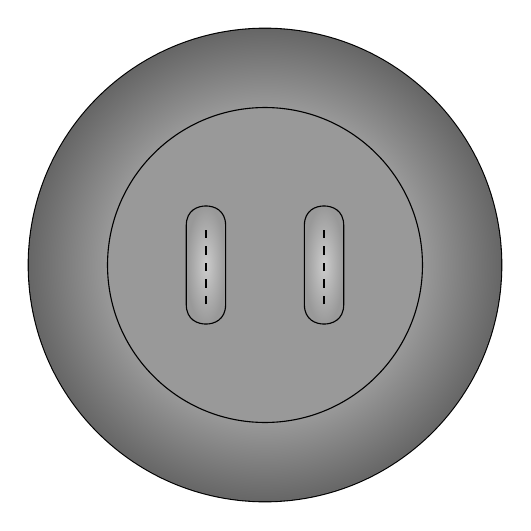
\begin{tikzpicture}
\draw[thick] (0, 0) circle (3);
\fill[outer color = black!60, inner color = white] (0, 0) circle (3);
\fill[color = black!40] (0, 0) circle (2);
\draw (0, 0) circle (2);
\filldraw[outer color = black!40, inner color=black!20] 
	(-0.75, -0.75) .. controls +(0.1, 0) and +(0, -0.2) ..
	(-0.5, -0.5) --
	(-0.5, 0.5) .. controls +(0, 0.2) and +(0.1, 0) ..
	(-0.75, 0.75) .. controls +(-0.1, 0) and +(0, 0.2) ..
	(-1, 0.5) -- 
	(-1, -0.5) .. controls +(0, -0.2) and +(-0.1, 0) ..
	(-0.75, -0.75);
\filldraw[outer color = black!40, inner color=black!20] 
	(0.75, -0.75) .. controls +(-0.1, 0) and +(0, -0.2) ..
	(0.5, -0.5) --
	(0.5, 0.5) .. controls +(0, 0.2) and +(-0.1, 0) ..
	(0.75, 0.75) .. controls +(0.1, 0) and +(0, 0.2) ..
	(1, 0.5) -- 
	(1, -0.5) .. controls +(0, -0.2) and +(0.1, 0) ..
	(0.75, -0.75);
\draw[thick, dashed] (-0.75, -0.5) -- (-0.75, 0.5);
\draw[thick, dashed] (0.75, -0.5) -- (0.75, 0.5);
\end{tikzpicture}


\end{document}
